\let\negmedspace\undefined
\let\negthickspace\undefined
\documentclass[journal,12pt,onecolumn]{IEEEtran}
\usepackage{cite}
\usepackage{amsmath,amssymb,amsfonts,amsthm}
\usepackage{algorithmic}
\usepackage{graphicx}
\graphicspath{{./figs/}}
\usepackage{textcomp}
\usepackage{xcolor}
\usepackage{txfonts}
\usepackage{listings}
\usepackage{enumitem}
\usepackage{mathtools}
\usepackage{gensymb}
\usepackage{comment}
\usepackage{caption}
\usepackage[breaklinks=true]{hyperref}
\usepackage{tkz-euclide} 
\usepackage{listings}
\usepackage{gvv}                                        
%\def\inputGnumericTable{}                                 
\usepackage[latin1]{inputenc}     
\usepackage{xparse}
\usepackage{color}                                            
\usepackage{array}                                            
\usepackage{longtable}                                       
\usepackage{calc}                                             
\usepackage{multirow}
\usepackage{multicol}
\usepackage{hhline}                                           
\usepackage{ifthen}                                           
\usepackage{lscape}
\usepackage{tabularx}
\usepackage{array}
\usepackage{float}
%\newtheorem{theorem}{Theorem}[section]
%\newtheorem{problem}{Problem}
%\newtheorem{proposition}{Proposition}[section]
%\newtheorem{lemma}{Lemma}[section]
%\newtheorem{corollary}[theorem]{Corollary}
%\newtheorem{example}{Example}[section]
%\newtheorem{definition}[problem]{Definition}
\begin{document}

\begin{center}
    \huge{XL: LIFE SCIENCES}\\
    \large{AI25BTECH11001 - Abhisek Mohapatra}\\
    \large{GRADUATE APTITUDE TEST IN ENGINEERING}
\end{center}
\textbf{General Aptitude}
\begin{enumerate}

\item Choose the most appropriate word from the options given below to complete the following sentence. 
	The principal presented the chief guest with a \rule{1cm}{0.15mm} as token of appreciation.
    \begin{enumerate}
		    \begin{multicols}{4}
		\item{ momento}
		\item {memento}
		\item {momentum}
		\item {moment}
		    \end{multicols}
    \end{enumerate}

\hfill{\textbf{GATE XL 2015}}

\item Choose the appropriate word/phrase, out of the four options given below, to complete the following sentence

	\textbf{Frogs}
    \begin{enumerate}
		    \begin{multicols}{4}
            \item croak
            \item roar
            \item hiss
            \item patter
		    \end{multicols}
    \end{enumerate}

\hfill{\textbf{GATE XL 2015}}
\item Choose the word most similar in meaning to the given word

	\textbf{Educe}
    \begin{enumerate}
		    \begin{multicols}{4}
            \item Exert
            \item Educate
            \item Extract
            \item Extend
		    \end{multicols}
    \end{enumerate}
\hfill{\textbf{GATE XL 2015}}
\item Operators $\Box$,$\diamondsuit$ and $\rightarrow$ are defined by: a$\Box b=\frac{a-b}{a+b};a \diamondsuit b = \frac{a+b}{a-b};a\rightarrow b = ab$. Find the value of $\brak{66\Box6}$ $\rightarrow$ $ \brak{66\diamondsuit6}$.
    \begin{enumerate}
		    \begin{multicols}{4}
            \item -2
            \item -1
            \item 1
            \item 2
		    \end{multicols}
    \end{enumerate}
\hfill{\textbf{GATE XL 2015}}
\item If log$_x$\brak{5/7}=-1/3, then the value of x is
    \begin{enumerate}
            \item 343/125
            \item 125/343
            \item -25/49
            \item -49/25
    \end{enumerate}
\hfill{\textbf{GATE XL 2015}}
\item The following question presents a sentence, part of which is underlined. Beneath the sentence you find four ways of phrasing the underlined part. Following the requirements of the standard written English, select the answer that produces the most effective sentence.

	Tuberculosis, together with its effects, \underline{ranks one of the leading causes of death} in India.
    \begin{enumerate}
            \item ranks as one of the leading causes of death
            \item  rank as one of the leading causes of death
            \item has the rank of one of the leading causes of death
            \item are one of the leading causes of death
    \end{enumerate}
\hfill{\textbf{GATE XL 2015}}
\item Read the following paragraph and choose the correct statement.

Climate change has reduced human security and threatened human well being. An ignored reality of human progress is that human security largely depends upon environmental security. But on the contrary, human progress seems contradictory to environmental security. To keep up both at the required level is a challenge to be addressed by one and all. One of the ways to curb the climate change may be suitable scientific innovations, while the other may be the Gandhian perspective on small scale progress with focus on sustainability.
    \begin{enumerate}
            \item Human progress and security are positively associated with environmental security.
            \item Human progress is contradictory to environmental security.
	\item Human security is contradictory to environmental security.  
            \item Human progress depends upon environmental security.
    \end{enumerate}
\hfill{\textbf{GATE XL 2015}}
\item Fill in the missing value
	\begin{figure}[h!]
	\centering
	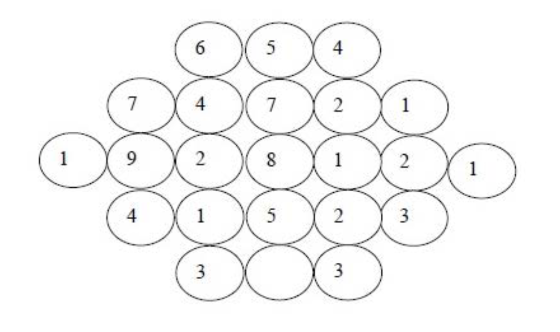
\includegraphics[width=10cm]{8}
	\caption*{}
	\label{fig:Q8}
	\end{figure}
\hfill{\textbf{GATE XL 2015}}
\item 
A cube of side 3 units is formed using a set of smaller cubes of side 1 unit. Find the proportion of the number of faces of the smaller cubes visible to those which are NOT visible
    \begin{enumerate}
		    \begin{multicols}{4}
            \item 1:4
            \item 1:3
            \item 1:2
            \item 2:3
		    \end{multicols}
    \end{enumerate}
\hfill{\textbf{GATE XL 2015}}
\item Humpty Dumpty sits on a wall every day while having lunch. The wall sometimes breaks. A person sitting on the wall falls if the wall breaks.

Which one of the statements below is logically valid and can be inferred from the above sentences?
    \begin{enumerate}
            \item Humpty Dumpty always falls while having lunch  
            \item Humpty Dumpty does not fall sometimes while having lunch
            \item Humpty Dumpty never falls during dinner
            \item When Humpty Dumpty does not sit on the wall, the wall does not break
    \end{enumerate}
\hfill{\textbf{GATE XL 2015}}


	\textbf{Chemistry}
\item The molecule having net \' non-zero dipole moment\' is
    \begin{enumerate}
		    \begin{multicols}{4}
            \item CCl$_4$
            \item NF$_3$
            \item CO$_2$
            \item BCl$_3$
		    \end{multicols}
    \end{enumerate}
\hfill{\textbf{GATE XL 2015}}
\item The Diels-Alder adduct from the reaction between cyclopentadiene and benzyne is
    \begin{enumerate}
		    \begin{multicols}{2}
	\begin{figure}[h!]
		\centering
            \item 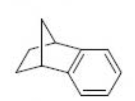
\includegraphics{12a}
		    \caption*{}
		\label{fig:Q12a}
	\end{figure}
	\begin{figure}[h!]
		\centering
            \item 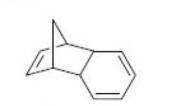
\includegraphics{12b}
		    \caption*{}
		\label{fig:Q12b}
	\end{figure}
	\begin{figure}[h!]
		\centering
	    \item 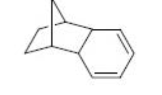
\includegraphics{12c}
		    \caption*{}
		\label{fig:Q12c}
	\end{figure}
	\begin{figure}[h!]
		\centering
            \item 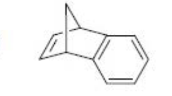
\includegraphics{12d}
		    \caption*{}
		\label{fig:Q12d}
	\end{figure}
		    \end{multicols}
    \end{enumerate}
\hfill{\textbf{GATE XL 2015}}
\item The number of possible enantiomeric pair(s) in HOOC-CH(OH)-CH(OH)-COOH is \rule{1cm}{0.15mm}.
\hfill{\textbf{GATE XL 2015}}
\item For the electrochemical reaction, Cu$^{2+}\textit{(aq)}+Zn\textit{(s)} \rightleftharpoons Cu(s) +Zn^{2+} \brak{aq}$ the equilibrium constant at 25 $25^{\circ} C$ is 1.7$\times 10 ^{37}$.The change in standard Gibbs free energy $\brak{\Delta G}$ for this reaction will be $(Given: R = 8.314JK ^ {- 1} mol ^{- 1} )$\rule{1cm}{0.15mm} kJ mol$^{-1}$ $(up \ to \ one \ decimal \ place)$.
\hfill{\textbf{GATE XL 2015}}
\item Among the following diagrams, the one that correctly describes a zero order reaction $(X \ product)$ is

$\brak{Given: \ [X]_0 =initial \ concentration \ of \ reactant \ X, \ [X] \ =  \ concentration \ of \ reactant \ X \ at \ time \ t \ and \ t_{1/2} = half-life \ period \ of \ reactant \ X}$
    \begin{enumerate}
	\begin{figure}[h!]
		\centering
	    \item 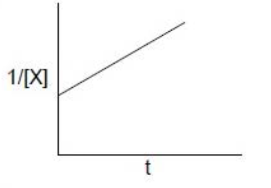
\includegraphics{15a}
		    \caption*{}
		\label{fig:Q15a}
	\end{figure}
	\begin{figure}[h!]
		\centering
	    \item 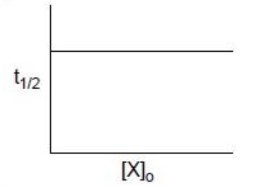
\includegraphics{15b}
		    \caption*{}
		\label{fig:Q15b}
	\end{figure}
	\begin{figure}[h!]
		\centering
	    \item 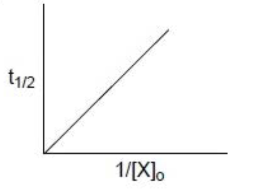
\includegraphics{15c}
		    \caption*{}
		\label{fig:Q15c}
	\end{figure}
	\begin{figure}[h!]
		\centering
	    \item 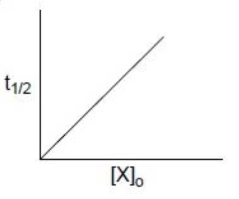
\includegraphics{15d}
		    \caption*{}
		\label{fig:Q15d}
	\end{figure}
    \end{enumerate}
\hfill{\textbf{GATE XL 2015}}
\item If the radius of first Bohr orbit is 0.53 $\AA$, then the radius of the third Bohr orbit is
    \begin{enumerate}
		    \begin{multicols}{4}
            \item 2.12 $\AA$
            \item 4.77 $\AA$
            \item 1.59 $\AA$
            \item 3.18 $\AA$
		    \end{multicols}
    \end{enumerate}
\hfill{\textbf{GATE XL 2015}}
\item If 50 mL of 0.02 M HCl is added to 950 mL of H$_2$O then the pH of the final solution will be \rule{1cm}{0.15mm}
\hfill{\textbf{GATE XL 2015}}
\item Stability of $[CrCl_6 ]^{3-} (X), [MnCl_6 ]^{3-} (Y) and [FeCl_6 ]^{3-} (Z)$ follows the order

	(Given: Atomic \ numbers \ of \ Cr \ = 24 \ Mn = 25 \ and \ Fe = 26 )    \begin{enumerate}
		    \begin{multicols}{4}
            \item $X > Y > Z $
            \item $X < Y < Z $
            \item $Y < X < Z $
            \item $X < Y = Z$ 
		    \end{multicols}
    \end{enumerate}
\hfill{\textbf{GATE XL 2015}}
\item Among the following pairs, the paramagnetic and diamagnetic species, respectively, are
    \begin{enumerate}
		    \begin{multicols}{4}
            \item CO and O$_2^-$
            \item NO and CO
            \item O$_2^{2-}$ and CO
            \item NO$^+ $ AND O$_2^-$
		    \end{multicols}
    \end{enumerate}
\hfill{\textbf{GATE XL 2015}}
\item In compounds K4$[Fe(CN)_6]-{-4}$ (P) and Fe(CO)s (Q), the iron metal centre is bonded to
    \begin{enumerate}
            \item C of CN$^-$ in P and C of CO in Q
            \item N of CN$^-$ in Pand C of CO in Q
            \item C of CN$^-$ in P and O of CO in Q
            \item N of CN$^-$ in P and O of CO in Q
    \end{enumerate}
\hfill{\textbf{GATE XL 2015}}
\item  Among the following reactions, the one that produces achiral alcohol (after hydrolysis) is

	
	\begin{figure}[h!]
		\centering
    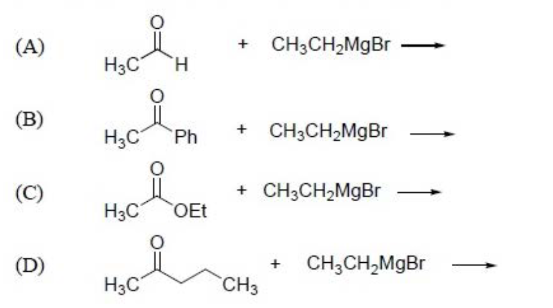
\includegraphics[width=10cm]{21}
		    \caption*{}
		\label{fig:Q21}
	\end{figure}
\hfill{\textbf{GATE XL 2015}}
\item The major product from the following reaction is
    
	\begin{figure}[h!]
    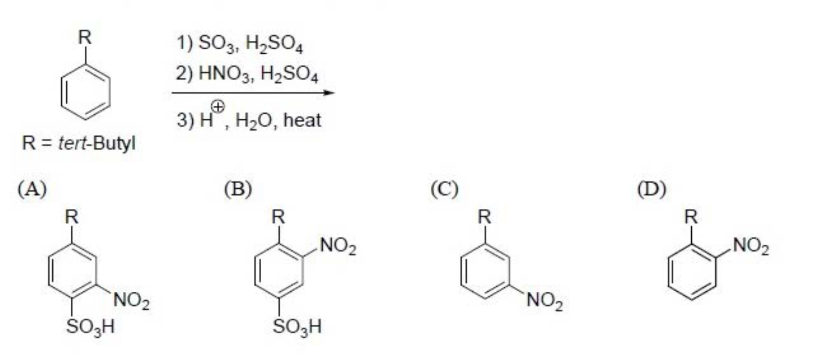
\includegraphics[width=15cm]{22}
		\centering
		    \caption*{}
		\label{fig:Q22}
	\end{figure}
\hfill{\textbf{GATE XL 2015}}
\item The order of resonance energy for the following molecules is
    
	\begin{figure}[h!]
		\centering
    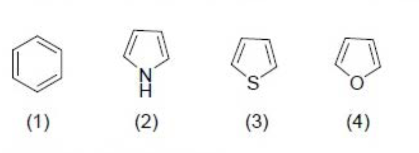
\includegraphics{23}
		    \caption*{}
		\label{fig:Q23}
	\end{figure}

	\begin{enumerate}
		    \begin{multicols}{2}
		    \item $ (1)>(3)>(2)>(4)$
		    \item $(1)>(3)>(4)> (2)$
		    \item $(1)> (4)>(2)> (3)$
		    \item $(1)>(3)>(4)> (2)$
		    \end{multicols}
    \end{enumerate}
\hfill{\textbf{GATE XL 2015}}
\item The molar enthalpy of vaporization for a liquid $(normal boiling point = 78.3 C) is 39 kJ mol^{-1}$. If the liquid has to boil at 25$\degree$C, the pressure must be reduced to Torr $(up to one decimal place)$.

	$(Given: R=8.314 JK mol, 1 atm = 760 Torr)$
\hfill{\textbf{GATE XL 2015}}
\item For the process, H$_2O$ $(l)$ $\leftrightarrow$ H$_2$O $(s)$ at 0$\degree C$ and 1 atm, the correct statement is
    \begin{enumerate}
		    \begin{multicols}{4}
            \item $\Delta S_{system}$ = 0
	    \item $\Delta S_{total} >$ 0
	    \item $\Delta S_{total}$ = 0
            \item $\Delta S_{total} <$ 0
		    \end{multicols}
    \end{enumerate}
\hfill{\textbf{GATE XL 2015}}
	

	\textbf{Biochemistry}
\item Which one of the following small molecules is a prerequisite for fatty acid oxidation?
    \begin{enumerate}
		    \begin{multicols}{4}
            \item Inositol
	    \item Choline
	    \item Carnitine
            \item Glycerol
		    \end{multicols}
    \end{enumerate}
\hfill{\textbf{GATE XL 2015}}
\item Which one of the following bases is NOT found in the T-arm of an aminoacyl t-RNA?
    \begin{enumerate}
            \item Dihydrouridine
	    \item Pseudouridine
	    \item Uracil
            \item Guanine
    \end{enumerate}
\hfill{\textbf{GATE XL 2015}}
\item Oxidation of one molecule of glucose via the glycerol-phosphate shuttle produces
    \begin{enumerate}
		    \begin{multicols}{2}
            \item 32 molecules of ATP
	    \item 32 molecules of NADPH
	    \item 30 molecules of ATP
            \item 30 molecules of NADPH
		    \end{multicols}
    \end{enumerate}
\hfill{\textbf{GATE XL 2015}}
\item Ribulose-5-phosphate epimerase is involved in which one of the following processes?
    \begin{enumerate}
            \item Glycolysis
	    \item TCA cycle
	    \item Glycosylation
            \item Pentose phosphate pathway
    \end{enumerate}
\hfill{\textbf{GATE XL 2015}}
\item Proteolytic enzymes are usually biosynthesized as large, inactive precursors known as
    \begin{enumerate}
		    \begin{multicols}{2}
            \item holoenzymes
	    \item zymogens
	    \item ribozyme
            \item apoenzymes
		    \end{multicols}
    \end{enumerate}
\hfill{\textbf{GATE XL 2015}}
\item The formation of a carbocation, also called an oxonium ion, occurs during the reaction catalyzed by
    \begin{enumerate}
		    \begin{multicols}{4}
            \item aldolase 
	    \item lysozyme
	    \item ribonuclease A
            \item carboxypeptidase
		    \end{multicols}
    \end{enumerate}
\hfill{\textbf{GATE XL 2015}}
\item Which one of the following amino acid substitutions is likely to cause the largest change in protein conformation?
    \begin{enumerate}
		    \begin{multicols}{4}
            \item Phe$\rightarrow$ Ile
	    \item Ser$\rightarrow$ Thr
	    \item Gin$\rightarrow$ Tyr
            \item Glu$\rightarrow$Val
		    \end{multicols}
    \end{enumerate}
\hfill{\textbf{GATE XL 2015}}
\item Which one of the following does NOT constitute the lipid moiety in lipid-linked membrane proteins?
        \begin{enumerate} 
		    \begin{multicols}{4}
            \item Palmitic acid
	    \item Farnesyl groups
	    \item Stearic acid
            \item Myristic acid
		    \end{multicols}
	\end{enumerate}
\hfill{\textbf{GATE XL 2015}}
\item A closed circular B-DNA of 4000 base pairs is negatively supercoiled by introduction of 4 writhes. The super helical density of the resultant DNA molecule will be
\hfill{\textbf{GATE XL 2015}}
\item Which one of the following is NOT a receptor tyrosine kinase?
    \begin{enumerate}
            \item Platelet derived growth factor receptor
	    \item Insulin like growth factor-1 receptor
	    \item Macrophage colony stimulating factor receptor
            \item Transforming growth factor $\beta$ receptor
    \end{enumerate}
\hfill{\textbf{GATE XL 2015}}
\item Match the entries in Column-1 with those in Column-2


	\begin{minipage}{0.5\textwidth}
		\begin{flushleft}
Column-1

P. Vitamin B1


Q. Carboxypeptidase


R TCA cycle


S. Reducing sugar

		\end{flushleft}
	\end{minipage}
	\begin{minipage}{0.5\textwidth}
		\begin{flushleft}
Column-2

1. Thiamine pyrophosphate

2. Aconitase

3. Sucrose

4. Zn

5. Riboflavin

6. Lactose

		\end{flushleft}
	\end{minipage}
    \begin{enumerate}
            \item P-1; Q-4, R-2, S-6
	    \item P-5; Q-1; R-2; S-3
	    \item P-1; Q-4; R-5; S-6
            \item P-5; Q-2; R-1; S-6
	\end{enumerate}
\hfill{\textbf{GATE XL 2015}}
\item The following table provides information about four proteins.
\vspace{0.2cm}
\begin{table}[H]
\begin{tabular}{|c|c|c|c|}
\hline
\text{Protein} & \text{Native mol.wt.\(Da\)}  &\text{pI} & \text{Type} \\
\hline
P & 32000 & 6.4&monomer \\
\hline
Q & 40000 & 8.5&homodimer \\
\hline
R & 25000 & 4.9&monodimer \\
\hline
S & 45000 & 8.5&homodimer \\
\hline
\end{tabular}

	\caption*{}
	\label{37}
\end{table}
Which one of the following options correctly identifies the order of elution in size exclusion chromatography and the increasing order of mobility in SDS polyacrylamide gel?
    \begin{enumerate}
	    \item Chromatrography SQPR; Electrophoresis: RPQS
	    \item Chromatrography: PRQS; Electrophoresis: PRQS
	    \item Chromatrography: RPQS, Electrophoresis: SQPR
            \item Chromatrography: SQPR, Electrophoresis: PRQS
    \end{enumerate}
\hfill{\textbf{GATE XL 2015}}
\item The predicted molar extinction coefficient at 280 nm for the peptide

	\textbf{GEEFHISFLLIMFGAWSTHMYRTYWFIHEMISTRY} is\rule{1cm}{0.15mm} M$^{-1}cm^{-1}$

Molar extinction coefficients for phenylalanine, tryptophan and tyrosine at 280 nm are 200, 5600 and 1400 M$^{-1}cm^{-1}$, respectively
\hfill{\textbf{GATE XL 2015}}
\item Match the contents of Column I with the most appropriate options in Column II
	

	\begin{minipage}{0.5\textwidth}
		\begin{flushleft}
Column I

P. Complement Clq

Q. L-Selectin

R. Membrane Attack Complex

S. T-Helper cells
		\end{flushleft}
	\end{minipage}
	\begin{minipage}{0.5\textwidth}
		\begin{flushleft}
Column II

1. CD34

ii. Complement CSb

im. Fc region of antibody

iv. Complement CSa

v. CD40L
		\end{flushleft}
	\end{minipage}

        \begin{enumerate} 
            \item P-iii; Q-v: R-iv, S-i
	    \item P-i Q-ii R-iv S-v
	    \item P-iii; Q-i R-ii S-v
            \item P-iv Q-v: R-iiS-i
	\end{enumerate}
\hfill{\textbf{GATE XL 2015}}
\item The value of $\Delta$G at 37$25^{\circ}C$ for the movement of Ca$^{2+}$ ions from the endoplasmic reticulum where [Ca$^{2+}$] is 1 mM to the cytosol where [Ca$^{2+}$] is 0.1 $\micro$M at -50 mV membrane potential is\rule{1cm}{0.15mm} kJ mol$^{-1}$.

	[R-8.314 JK mol$^{-1}$ and 1 Faraday = 96500 Coulombs]
\hfill{\textbf{GATE XL 2015}}
\item 

	\begin{figure}[h!]
		\centering
    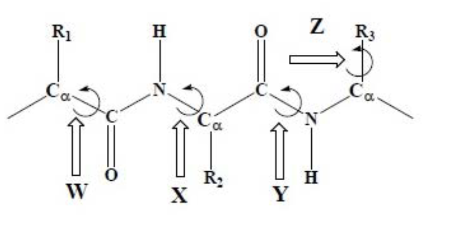
\includegraphics{41}
		    \caption*{}
		\label{fig:Q41}
	\end{figure}

Which of the following identifies the correctly matched pairs?
        \begin{enumerate} 
            \item W-iii X-i Y-iv, Z-ii
	    \item W-i X-iii, Y-iv, Z-ii
	    \item W-i X-iii: Y-ii Z-iv
            \item W-iii; X-i Y-ii Z-iv
	\end{enumerate}
\hfill{\textbf{GATE XL 2015}}
\item Which of the following statements is/are INCORRECT about hemoglobin (Hb)?

I. Hb demonstrates higher oxygen carrying capacity compared to myoglobin

II. There is covalent bonding between the four subunits of Hb

III. During deoxygenation the loss of the first oxygen molecule from oxygenated Hb promotes the dissociation of oxygen from the other subunits
    \begin{enumerate}
            \item II
	    \item II and III
	    \item I and III
            \item III
	\end{enumerate}
\hfill{\textbf{GATE XL 2015}}
\item A 1.2 kb DNA fragment was used as a template for PCR amplification using primers P1, P2, P3 and P4 as shown in the scheme below. The annealing positions of primers on the template are indicated by numbers. Primers P2 and P3 contain single base mismatches as indicated by filled triangles.
	
	\begin{figure}[h!]
		\centering
    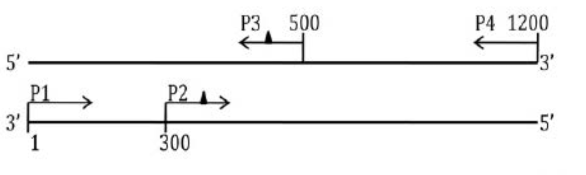
\includegraphics[width=\columnwidth]{43}
		    \caption*{}
		\label{fig:Q43}
	\end{figure}
PCR was performed using primer pair P1 and P3 in one vial and P2 and P4 in another vial. The purified PCR products from the two vials were mixed and subjected to another round of PCR with primers P1 and P4. The final PCR product will correspond to a

    \begin{enumerate}
            \item .2 kb wild type DNA
	    \item  1.2 kb DNA with two point mutations
	    \item  0.9 kb DNA with one point mutation
            \item 0.5 kb DNA with one point mutation
    \end{enumerate}
\hfill{\textbf{GATE XL 2015}}
\item A cell suspension was subjected to membrane disruption followed by differential centrifugation to fractionate the cellular components.

    
Match the centrifugal conditions in Column I to the appropriate subcellular components in Column
\begin{minipage}{0.5\textwidth}
	\begin{flushleft}
Column I

P. 1000 g, 10 min

Q. 20000g 30 min

R. 80000 g, 1 hour

S. 150000 g, 3 hours
	\end{flushleft}
\end{minipage}
\begin{minipage}{0.5\textwidth}
	\begin{flushleft}
Column II

1. Microsomes and small vesicles

ii. Ribosomes

in. Nuclei

iv. Lysosomes and peroxisomes
	\end{flushleft}
\end{minipage}
    \begin{enumerate}
            \item P - iii, Q-iv, R-i, S-ii
            \item P - i, Q-iv, R-iii, S-ii
            \item P - iii, Q-iv, R-ii, S-i
            \item P - ii, Q-i, R-iv, S-iii
    \end{enumerate}
\hfill{\textbf{GATE XL 2015}}
\item Given below are the maps of a 1200 base pairs (bp) long DNA insert and a 3000 bp expression vector. The BamHI (B) and HindIII (H) restriction sites and DNA length between them are indicated in base pairs.

	\begin{figure}[h!]
		\centering
	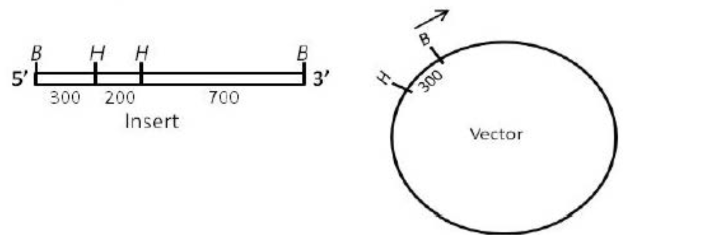
\includegraphics[width=\columnwidth]{45}
		    \caption*{}
		\label{fig:Q45}
	\end{figure}

The insert is cloned into the vector at the BamHI site and the desired orientation is shown by the arrow. After cloning, the orientation of the insert in the recombinant plasmid is tested by complete HindIII digestion followed by agarose gel electrophoresis. Which one of the following band patterns reveals the correct orientation of the insert in the construct?
    
	\begin{figure}[h!]
		\centering
	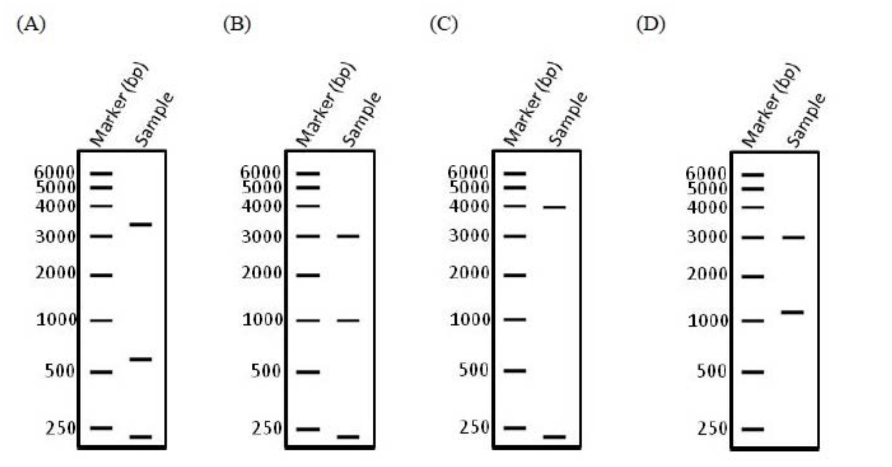
\includegraphics[width=\columnwidth]{45op}
		    \caption*{}
		\label{fig:Q45op}
	\end{figure}
\hfill{\textbf{GATE XL 2015}}
	

	\textbf{Botany}
\item Nuclear membrane is absent in
    \begin{enumerate}
            \item Chlamydomonas
	    \item Nostoc
	    \item Volvox
            \item Chlorella
    \end{enumerate}
\hfill{\textbf{GATE XL 2015}}
\item An organized and differentiated cell having cytoplasm but no nucleus is found in
    \begin{enumerate}
            \item Companion cell
	    \item Xylem parenchyma
	    \item Sieve tube element
            \item Phloem parenchyma
    \end{enumerate}
\hfill{\textbf{GATE XL 2015}}
\item Double haploids in plants can be induced by
    \begin{enumerate}
            \item Mitomycin-C
	    \item Mirin
	    \item Colchicine
            \item 5-Azacytidine
    \end{enumerate}
\hfill{\textbf{GATE XL 2015}}
\item During fatty acid biosynthesis, the first intermediate malonyl-CoA is formed from 
    \begin{enumerate}
            \item Acetyl-CoA and bicarbonate
	    \item Two acetyl-CoA molecules
	    \item Acetyl-CoA and biotin
	    \item  Palmitoyl CoA and acyl-carrier protein (ACP)
	\end{enumerate}
\hfill{\textbf{GATE XL 2015}}
\item  Which of the following techniques is NOT applicable for evaluating the expression of a transgene?
        \begin{enumerate} 
            \item Northern blot
	    \item RT-PCR
	    \item Western blot
            \item Southern blot
	\end{enumerate}
\hfill{\textbf{GATE XL 2015}}
\item Identify the CORRECT family possessing the following characters presence of glucosinolates, tetradynamous stamens, superior ovary with parietal placentation and siliqua type fruit
        \begin{enumerate} 
            \item Brassicaceae
	    \item Capparidaceae
	    \item Fumariaceae
            \item Papavaraceae
    \end{enumerate}
\hfill{\textbf{GATE XL 2015}}
\item Which of the following reduces the transpiration rate when applied to aerial parts of plants?
    \begin{enumerate}
            \item Phosphon-D
	    \item Paraquat
	    \item Phenyl mercuric acetate
            \item Valinomycin
    \end{enumerate}
\hfill{\textbf{GATE XL 2015}}
\item A tube like membrane structure that forms the connection between the endoplasmic reticulum of neighboring cells through plasmodesmata is
    \begin{enumerate}
            \item Desmotubule
	    \item Desmosome
	    \item Dictyosome
            \item Microtubule  
    \end{enumerate}
\hfill{\textbf{GATE XL 2015}}
\item Which one of the followings is NOT a cryoprotectant for plant tissue?
    \begin{enumerate}
            \item Dimethyl sulfoxide
	    \item Glycerol
	    \item Ethylene glycol
            \item Liquid nitrogen
    \end{enumerate}
\hfill{\textbf{GATE XL 2015}}
\item Two similar holotypes are called
    \begin{enumerate}
            \item Monotype
	    \item Neotype
	    \item Isotype
            \item Syntype
    \end{enumerate}
\hfill{\textbf{GATE XL 2015}}
\item A cross was made berween AABBCCDDEE and aabbccddee. The resultants F, were selfed. Applying Mendelian principle, PREDICT the proportion of phenotype showing all the recessive characters in F; generation.
    \begin{enumerate}
            \item 1/64
	    \item 1/256
	    \item 1/512
            \item 1/1024
    \end{enumerate}
\hfill{\textbf{GATE XL 2015}}
\item Identify the CORRECT statements with respect to functioning of ecosystem.

P. A food chain is a series of organisms, each one feeding on the organism succeeding it

Q. Food web presents a complete picture of the feeding relationships in any given ecosystem

R. In ecosystem, energy flows in unidirectional way, whereas nutrients flow in cyclic fashion

S. In biogeochemical cycles, nutrients do not alternate between organisms and environment
    \begin{enumerate}
            \item P,Q
	    \item P, R
	    \item R, S
            \item Q, R
    \end{enumerate}
\hfill{\textbf{GATE XL 2015}}
\item Match the name of the diseases with their causal organisms.

\begin{minipage}{0.5\textwidth}
	\begin{flushleft}
Disease

P. Loose smut of wheat

Q. Wart disease of potato

R. Panama disease of banana

S. Tikka disease of groundnut

	\end{flushleft}
\end{minipage}
\begin{minipage}{0.5\textwidth}
	\begin{flushleft}
Causal Organism

1. Cercospora personata 2. Alternaria solani

3. Synchytrium endobioticum

4. Ustilago tritici

5. Fusarium oxysporum

6. Erwinia amylovora
	\end{flushleft}
\end{minipage}

    \begin{enumerate}
            \item P-6, Q-4, R-3, S-2
	    \item P-4. Q-6, R-1, S-3
	    \item P-4. Q-3, R-5, S-1
            \item P-2, Q-3, R-2, S-6
    \end{enumerate}
\hfill{\textbf{GATE XL 2015}}
\item Match the plant products with their sources and the plant parts from which they are obtained,

\begin{minipage}{0.3\textwidth}
	\begin{flushleft}
Product

P. Annatto

Q. Cutch

R. Henna

S. Alizarin

	\end{flushleft}
\end{minipage}
\begin{minipage}{0.3\textwidth}
	\begin{flushleft}
Source

1. Acacia catechu

3. Bixa orellana

i. Root

4. Lawsonia inermis

	\end{flushleft}
\end{minipage}
\begin{minipage}{0.3\textwidth}
	\begin{flushleft}
Plant part

1. Seed

2. Rubia tinctorum

n. Leaf
IV. Stem
	\end{flushleft}
\end{minipage} 
    \begin{enumerate}
            \item P-3-n, Q-4-1, R-2-m, S-1-iv
	    \item  P-3-1, Q-1-1v, R-4-n, S-2-m
	    \item P-2-ii. Q-1-in. R-4-iv, S-3-1
            \item P-4-ii, Q-3-iv, R-1-ii, S-2-4
    \end{enumerate}
\hfill{\textbf{GATE XL 2015}}
\item Match the floral structures with the families and representative plant species.

\begin{minipage}{0.3\textwidth}
	\begin{flushleft}
Floral structure
P. Gynostegium

Q. Gynostemium

R. Gynobasic style

S. Gynophore

	\end{flushleft}
\end{minipage}
\begin{minipage}{0.3\textwidth}
	\begin{flushleft}
Family


1. Orchidaceae

2. Lamiaceae

3. Capparidaceae

4. Asclepiadaceae

	\end{flushleft}
\end{minipage}
\begin{minipage}{0.3\textwidth}
	\begin{flushleft}
Plant
1. Ocimum sanctum

ii. Cleome gynandra

in. Calotropis procera

iv. Vanilla planifolia
	\end{flushleft}
\end{minipage}
    \begin{enumerate}
	\item P-2-i, Q-3-iii, R-4-ii, s-1-iv            
	\item P-3-ii, Q-4-i, R-2-iii, s-1-iv            
	\item P-4-iii, Q-1-iv, R-2-i, s-3-ii            
	\item P-4-ii, Q-2-iii, R-1-iv, s-3-i            
    \end{enumerate}
\hfill{\textbf{GATE XL 2015}}
\item  Identify the INCORRECT statements with respect to plastid transformation.

P. Antibiotic used for selection of trasplastomic plant is spectinomycin

Q. Chances of gene escape from transplastomic plants are high

S. Levels of transgene expression are low

R. Microprojectile bombardment is the method of DNA delivery
    \begin{enumerate}
            \item P,R
	    \item P,Q
	    \item Q,S
            \item R,S
    \end{enumerate}
\hfill{\textbf{GATE XL 2015}}
\item Which of the following statements are TRUE with regard to the similarities between Crassulacean.

	Acid Metabolism (CAM) and C$_4$, cycle?

P. Stomata open during night and remain closed during the day

Q. PEPcase is the carboxylating enzyme to form C$_4$ acid

R. C, acid is decarboxylated to provide CO$_2$ for C$_3$, cycle

S. Kranz anatomy is predominant in both CAM and C$_4$ plants
    \begin{enumerate}
            \item P,S
	    \item Q,S
	    \item P,Q
            \item R,S
    \end{enumerate}
\hfill{\textbf{GATE XL 2015}}
\item With respect to germination of seeds, the CORRECT sequence of events is

P. Seed imbibes water

Q. Mobilization of starch reserve to embryo

R. Diffusion of gibberellin from embryo to aleurone layer

S. Synthesis of a-amylase in the aleurone layer
    \begin{enumerate}
            \item P. Q. S. R
	    \item R. P. Q. S
	    \item P. R. S. Q
            \item R. Q. P. S
    \end{enumerate}
\hfill{\textbf{GATE XL 2015}}
\item 
Identify the CORRECT statements with regard to the function of plant hormones

P. ABA is synthesized from chorismate and promotes viviparous germination

Q. Auxin induces acidification of cell wall followed by turgour-induced cell expansion

R. Gibberellin-reponsive genes become activated by the repression of DELLA protein

S. Cytokinin regulates the G$_2$ to M transition in the cell cycle
    \begin{enumerate}
            \item P,Q
	    \item Q,R
	    \item Q,S
            \item P,R
    \end{enumerate}
\hfill{\textbf{GATE XL 2015}}
\item Statements given below are either TRUE (T) or FALSE (F). Find the correct combination

P. Somatic embryo is umpolar in nature

Q. Heterokaryon can be selected using a fluorescence-activated cell sorter (FACS)

R. The term somaclonal variation is coined by Larkin and Scowcroft

S. Differentiation of shoot buds during in vitro culture is known as somatic embryogenesis
    \begin{enumerate}
            \item  P-T, Q-F. R-T. S-F
	    \item  P-F. Q-T. R-F. S-T
	    \item P-T, Q-F. R-F, S-T
            \item P-F. Q-T, R-T, S-F
    \end{enumerate}
\hfill{\textbf{GATE XL 2015}}
\item Lophotrichous bacteria have
    \begin{enumerate}
            \item one flagellum
	    \item a cluster of flagella at one or both ends
	    \item flagella that are spread evenly over the whole surface
            \item a single flagellum at each pole
    \end{enumerate}
\hfill{\textbf{GATE XL 2015}}
\item In aerobic respiration, the final electron acceptor is
    \begin{enumerate}
            \item hydrogen
	    \item nitrogen
	    \item sulfur
            \item oxygen
    \end{enumerate}
\hfill{\textbf{GATE XL 2015}}
\item A process in which fatty acids are shortened by two carbons at a time resulting in release of acetyl-
CoA is known as
    \begin{enumerate}
            \item photophosphorylation
	    \item carboxylation
	    \item B-oxidation
            \item oxidative phosphorylation
    \end{enumerate}
\hfill{\textbf{GATE XL 2015}}
\item  Limulus Amoebocyte Lysate (LAL) assay is used to identify the presence of
    \begin{enumerate}
            \item endotoxin
	    \item exotoxin
	    \item anthrax toxin
            \item tetanus toxin
    \end{enumerate}
\hfill{\textbf{GATE XL 2015}}
\item Match scientists in Group I with terms related to their major scientific contributions in Group II

Group I

(P) Sanger

(Q) Watson and Crick

(R) Waksman

(S) Bordet
Group II

(1) DNA double helix structure

(1) DNA sequencing

(in) Complement

(iv) Streptomycin

(v) Immune tolerance
    \begin{enumerate}
            \item 
	    \item 
	    \item 
            \item 
    \end{enumerate}
\hfill{\textbf{GATE XL 2015}}
\item Base-pair substitutions caused by the chemical mutagen ethyl methane sulfonate are a result of
    \begin{enumerate}
            \item hydroxylation
	    \item alkylation
	    \item deamination
            \item intercalation
    \end{enumerate}
\hfill{\textbf{GATE XL 2015}}
\item  The classical way of representing taxonomic hierarchy of living organisms in ASCENDING

ORDER is
    \begin{enumerate}
            \item genus, species, class, order, family
	    \item genus, species, class, order, family
	    \item species, genus, family, order, class
            \item genus, species, order, class, family
    \end{enumerate}
\hfill{\textbf{GATE XL 2015}}
\item Of the following, the most effective method to kill bacterial endospores is 
    \begin{enumerate}
            \item moist heat sterilization
	    \item UV irradiation
	    \item filtration
            \item pasteurization
    \end{enumerate}
\hfill{\textbf{GATE XL 2015}}
\item The class of enzymes, which catalyze addition of groups to double bonds and non-hydrolytic removal of chemical groups, is
    \begin{enumerate}
            \item oxidoreductase
	    \item transferase
	    \item hydrolase
            \item lyase
    \end{enumerate}
\hfill{\textbf{GATE XL 2015}}
\item Anammox organisms carry out
    \begin{enumerate}
            \item anaerobic reduction of NO
	    \item anaerobic oxidation of NH 
	    \item aerobic oxidation of NH
            \item aerobic oxidation of NO
    \end{enumerate}
\hfill{\textbf{GATE XL 2015}}
\item Which combination of the following statements about specialized transduction is TRUE?

	(P) Specialized transducing phages can transport only certain genes between bacteria

(Q) Specialized transducing phages can transport any gene between bacteria

(R) Phage P22 is a specialized transducing phage

(S) Phage lambda (2) is a specialized transducing phage
    \begin{enumerate}
            \item P and S only
	    \item Q and R only
	    \item Q and S only
            \item P and R only
    \end{enumerate}
\hfill{\textbf{GATE XL 2015}}
\item Which combination of profiles in the following figure accurately represents the transport rate of glycerol and oxygen into E. coli cells as a function of their extracellular concentration?


	\begin{figure}[h!]
		\centering
	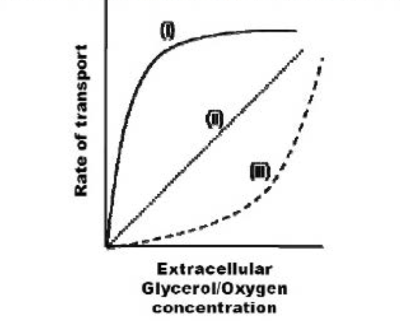
\includegraphics[width=10cm]{77}
		    \caption*{}
		\label{fig:Q77}
	\end{figure}
    \begin{enumerate}
	    \item glycerol-(ii) and oxygen-(iii)
	    \item glycerol-(ii) and oxygen-(i)
	    \item glycerol-(iii) and oxygen-(i)
	    \item glycerol-(i) and oxygen-(ii)
    \end{enumerate}
\hfill{\textbf{GATE XL 2015}}
\item Which one of the following about the standard free energy change $(\Delta G)$ and the equilibrium constant $(K_{eq})$ of an exergonic reaction, at pH 7.0, is TRUE?
    \begin{enumerate}
            \item $\Delta G$ is positive and K$_{eq}$ 15 less than one
	    \item $\Delta G$ is negative and K$_{eq}$ is less than one
	    \item $\Delta G$ is negative and K$_{eq}$ is greater than one
            \item $\Delta G$ is positive and K$_{eq}$ is greater than one
    \end{enumerate}
\hfill{\textbf{GATE XL 2015}}
\item An oil immersion objective of a light microscope has a numerical aperture of 1.25. Using the Abbé equation, the maximum theoretical resolving power $(in nm)$ of the microscope with this objective and blue light $(wavelength=450 nm)$ is

\hfill{\textbf{GATE XL 2015}}
\item The working volume (in liter) of a chemostat with 0.1 h$^{-1}$ dilution rate and 100 ml/h feed flow rate 15
\hfill{\textbf{GATE XL 2015}}
\item If the decimal reduction time for spores of a certain bacterium at 121$\degree$C is 12 seconds, the time required (in minutes) to reduce 10$^{10}$ spores to one spore by heating at 121$\degree$C is
\hfill{\textbf{GATE XL 2015}}
\item	The doubling time (in minutes) of a bacterium with a specific growth rate of 2.3 h$^{-1}$ in 500 ml of growth medium is
\hfill{\textbf{GATE XL 2015}}
\item
	A bacterial culture is grown using 2.0 mg/ml fructose as the sole source of carbon and energy. The bacterial biomass concentrations immediately after inoculation and at the end of the growth phase are 0.1 mg/ml and 0.9 mg/ml, respectively. Assuming complete utilization of the substrate, the bacterial growth yield (1) on fructose is 
        
\hfill{\textbf{GATE XL 2015}}
\item  The volume (in ml) of a 1.0 mg/ml stock solution of ampicillin to be added to 0.1 liter of growth medium for achieving a final ampicillin concentration of 50 $\micro$g/ml is
\hfill{\textbf{GATE XL 2015}}
\item An E. coli strain is grown initially on glucose as the sole carbon source. Upon complete consumption of glucose following 12 h of growth, lactose is added as the sole carbon source and the strain is further grown for 12 h. Assuming that the E. coli strain has a functional wild type lac operon, which one of the following profiles is the most ACCURATE representation of B-galactosidase $(B-gal)$ expression $(in arbitrary units)$?
	\begin{figure}[h!]
		\centering
	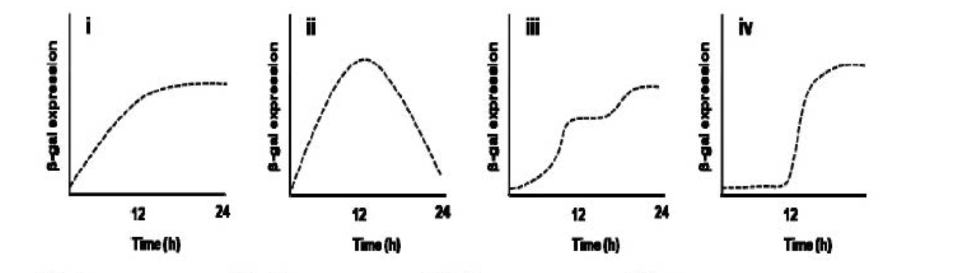
\includegraphics[width=15cm]{85}
		    \caption*{}
		\label{fig:Q85}
	\end{figure}
    \begin{enumerate}
            \item i
	    \item ii
	    \item iii
            \item iv
    \end{enumerate}
\hfill{\textbf{GATE XL 2015}}
	
	\textbf{Zoology}
\item  The term "paedomorphosis" refers to
    \begin{enumerate}
            \item Accelerated reproductive development as compared to somatic development
	    \item A transient stage in the developmental event
	    \item  Two independent structures resembling each other, yet performing different functions
            \item A form of mimicry
    \end{enumerate}
\hfill{\textbf{GATE XL 2015}}
\item Which one of the following statements is TRUE when determining the age of a fossil using carbon dating?
    \begin{enumerate}
            \item Carbon dating is based on carbon-13 to carbon-12 ratio in fossils
	    \item Carbon dating is useful for determining the age of only fossils older than 100,000 years
	    \item Older the fossil, lesser the carbon-14 to carbon-12 ratio
            \item Older the fossil, lesser the carbon-12 to carbon-14 ratio
    \end{enumerate}
\hfill{\textbf{GATE XL 2015}}
\item Constitutive enzymes are
    \begin{enumerate}
            \item Induced by effector molecules
	    \item Repressed by repressors
	    \item Encoded by sequences that occur as part of an operon
            \item Always produced in the cell
    \end{enumerate}
\hfill{\textbf{GATE XL 2015}}
\item Which one of the following is a function of intermediate filaments?
    \begin{enumerate}
            \item Chromosome movement during the cell division
	    \item Cytoplasmic streaming
	    \item Formation of tight junctions
            \item Anchorage of the nucleus
    \end{enumerate}
\hfill{\textbf{GATE XL 2015}}
\item Which one of the following statements is FALSE with respect to phospholipids?
    \begin{enumerate}
            \item  Phospholipids have amphipathic character
	    \item  Phospholipids form the lipid bilayer of the cell membrane
	    \item Phospholipids form micelles in living systems
            \item Some phospholipid molecules may contain a double bond in hydrophobic tails
    \end{enumerate}
\hfill{\textbf{GATE XL 2015}}
\item Which one of the following organs is INCORRECTLY paired with its function?
    \begin{enumerate}
            \item  Intestinal villi - absorption
	    \item Epiglottis - closure of larynx
	    \item Gall bladder - carbohydrate digestion
            \item Parietal cells - hydrochloric acid
    \end{enumerate}
\hfill{\textbf{GATE XL 2015}}
\item Where do B lymphocytes acquire immune competence?
    \begin{enumerate}
            \item Thymus 
	    \item Bone Marrow
	    \item Lymph nodes
            \item Spleen
    \end{enumerate}
\hfill{\textbf{GATE XL 2015}}
\item Which one of the following life cycle stages of Plasmodium falciparum is infectious?
    \begin{enumerate}
            \item Sporozoite
	    \item Cryptozoite
	    \item Merozoite
            \item Trophozoite
    \end{enumerate}
\hfill{\textbf{GATE XL 2015}}
\item What is the role of the notochord during organogenesis in a vertebrate embryo?
    \begin{enumerate}
            \item Signaling the development of placenta
	    \item  Induction of neural plate formation
	    \item Stimulation of the umbilical chord formation
            \item Suppression of the development of extra-embryonic membranes
    \end{enumerate}
\hfill{\textbf{GATE XL 2015}}
\item  The behavior of young ducks following their mother is known as
    \begin{enumerate}
            \item Imprinting
	    \item Innate behavior
	    \item Habituation
            \item Mimicry
    \end{enumerate}
\hfill{\textbf{GATE XL 2015}}
\item Match the species names with class names

	\begin{minipage}{0.5\textwidth}
		\begin{flushleft}
P. Calotes versicolor

Q. Periplaneta americana

R. Glyphidrilus birmancus

S. Clarias batracus

	\end{flushleft}
	\end{minipage}
	\begin{minipage}{0.5\textwidth}\begin{flushleft}
1. Insecta

11. Reptilia

III. Actinopterygi

iv. Clitellata

	\end{flushleft}
	\end{minipage}
    \begin{enumerate}
		\item P-1, Q-1, R-IV, S-m
	    \item P-1: Q-11, R-1; S-1V
	    \item P-11, Q-1, R-m; S-iv
            \item P-111, Q-1; R-11; S-1V
    \end{enumerate}
\hfill{\textbf{GATE XL 2015}}
\item A population of spotted deer found in a national forest is in Hardy-Weinberg equilibrium. For a particular genetic locus in this deer species, only two alleles A and a are possible. If the frequency of the Aa allele in this population is 0.6, and the frequency of the a allele is 0.4, what will be the frequency of the geotype Aa?
    \begin{enumerate}
            \item 0.24
	    \item 0.48
	    \item 0.96
            \item 1.6
    \end{enumerate}
\hfill{\textbf{GATE XL 2015}}
\item In \textit{Drosophila}, the gene for eye colour is present on the X chromosome. When a red-eyed female was mated with a white-eyed male, a total of 100 progeny were obtained 50 females and 50 males. Of the 50 females, 25 were red-eyed, and 25 were white-eyed. How many of the male progeny were red-eyed?
    \begin{enumerate}
            \item 0
	    \item 10
	    \item 20
            \item 25
    \end{enumerate}
\hfill{\textbf{GATE XL 2015}}
\item  Defect in poly-A tail formation in eukaryotic mRNA leads to
    \begin{enumerate}
            \item  Increased translation of the resulting mRNA
	    \item Decreased translation of the resulting mRNA
	    \item Premature transcription termination
            \item  Decreased mRNA stability
    \end{enumerate}
\hfill{\textbf{GATE XL 2015}}
\item Assuming equal frequency for all 4 nucleotides (G, A, T, C), how many EcoRI recognition sites (GAATTC) are possible in a bacterial artificial chromosome of 100,000 base pairs?
    \begin{enumerate}
            \item 6
	    \item 12
	    \item 24
            \item 48
    \end{enumerate}
\hfill{\textbf{GATE XL 2015}}
\item  Choose the correct option that shows pairing of the organelle to its function



	\begin{minipage}{0.5\textwidth}\begin{flushleft}
P. Smooth endoplasmic reticulum.

Q. Peroxisome

R. Golgi apparatus

S. Endosome
	\end{flushleft}
	\end{minipage}
	\begin{minipage}{0.5\textwidth}\begin{flushleft}
1. Internalization of receptors

11. Protein secretion

ii. Membrane biogenesis 

iv. Breakdown of fatty acids
	\end{flushleft}
	\end{minipage}
    \begin{enumerate}
            \item P-i;Q-ii;R-iii;S-iv
            \item P-i;Q-iii;R-ii;S-iv
            \item P-iii;Q-iv;R-ii;S-i
            \item P-ii;Q-iii;R-iv;S-i
    \end{enumerate}
\hfill{\textbf{GATE XL 2015}}

\item Choose the correct option based on your understanding of the circulatory system

	\begin{minipage}{0.5\textwidth}\begin{flushleft}
P. Open circulatory system

Q. Closed circulatory system

R. Three chambered heart

S. Two chambered heart
	\end{flushleft}
	\end{minipage}
	\begin{minipage}{0.5\textwidth}\begin{flushleft}
		i. Fish

		ii. Frog

		iii. Earthworm

		iv. Grasshopper

	\end{flushleft}
	\end{minipage}



    \begin{enumerate}
            \item P-iv;Q-iii;R-ii;S-i
            \item P-iv;Q-i;R-ii;S-iii
            \item P-i;Q-iv;R-ii;S-iii
            \item P-i;Q-iii;R-iv;S-ii
    \end{enumerate}



\hfill{\textbf{GATE XL 2015}}
\item  The popular birth control pills for women have a combination of synthetic forms of estradiol and

progesterone. Which one of the following statements is INCORRECT with regard to their function as contraceptive?
    \begin{enumerate}
            \item  The pills inhibit the release of GnRH leading to inhibition of gonadotropin-stimulated ovarian function
	    \item  They act directly on the pituitary gland to inhibit gonadotropin surges
	    \item The low dose of estradiol in the pill inhibits the release of FSH, and thus blocks ovulation
            \item The synthetic forms of estradiol and progesterone bring about their effects by binding to their respective intracellular receptors
    \end{enumerate}


\hfill{\textbf{GATE XL 2015}}
\item Which one of the following is consistent with the germplasm theory of August Weismann?
    \begin{enumerate}
            \item Regulative development observed in frog embryos
	    \item Mosaic development observed in tunicates
	    \item Normal embryonic development of embryos formed by somatic nuclear transfer
            \item Ability of differentiated cells to form pluripotent stem cells under certain conditions
    \end{enumerate}



\hfill{\textbf{GATE XL 2015}}
\item Which one of the following statements DOES NOT explain altruism?
    \begin{enumerate}
            \item Altruism reduces the fitness of the individual that displays this behavior
	    \item Altruism increases the fitness of other individuals in the population
	    \item Altruism reduces the fitness of the individual that displays this behavior and at the same time
increases the fitness of other individuals in the population
            \item  Altruistic behavior helps the individual escape from predators
    \end{enumerate}


\hfill{\textbf{GATE XL 2015}}
	

	\textbf{Food Technology}
\item Standard pasteurization protocol for milk is adequate for destroying
    \begin{enumerate}
            \item Clostridium sporogenes.
	    \item Bacillus cereus
	    \item Clostridium batulinum
            \item Listeria monocytogenes
    \end{enumerate}


\hfill{\textbf{GATE XL 2015}}
\item Which one of the following is NOT a component of an evaporator?
    \begin{enumerate}
            \item Heat exchanger
	    \item  Vacuum separator
	    \item Condenser
            \item Cyclone separator
    \end{enumerate}
\hfill{\textbf{GATE XL 2015}}
\item Among the following animal foods, the fat content is least in
    \begin{enumerate}
            \item Beef
	    \item Chicken meat
	    \item Pork
            \item Lamb flesh
    \end{enumerate}
\hfill{\textbf{GATE XL 2015}}
\item The enzyme that hydrolyzes starch to maltose is
    \begin{enumerate}
            \item $\alpha$-amylase
	    \item glucoamylase
	    \item $\beta$-amylase
            \item cyclodextrin glucanotransferase
    \end{enumerate}
\hfill{\textbf{GATE XL 2015}}
\item Which one of the following is NOT enriched in endosperm during parboiling of paddy?
    \begin{enumerate}
            \item Thiamine
	    \item Niacin
	    \item Iron
            \item Fat
    \end{enumerate}
\hfill{\textbf{GATE XL 2015}}
\item Heat-treated legume seed proteins are more digestible than those of untreated legume seed proteins due to
    \begin{enumerate}
            \item reaction of reducing sugars with e-amino group of lysine
	    \item increased binding of lectins to intestinal mucosal cells
	    \item thermolabile nature of lectins and Kunitz-type protease inhibitors 
            \item thermolabile nature of Bowman-Birk type of inhibitor
    \end{enumerate}
\hfill{\textbf{GATE XL 2015}}
\item What is the percent relative humidity at which both the dry bulb and wet bulb thermometers would record equal temperatures?
    \begin{enumerate}
            \item 0
	    \item 10
	    \item 50
            \item 100
    \end{enumerate}
\hfill{\textbf{GATE XL 2015}}
\item How many fold would the g-number of a centrifuge increase by doubling both the spinning speed and bowl diameter?
    \begin{enumerate}
            \item 2
	    \item 4
	    \item 8
            \item 16
    \end{enumerate}
\hfill{\textbf{GATE XL 2015}}
\item Prolonged fermentation of cocoa seeds lead to "off-taste" due to the release of
    \begin{enumerate}
            \item glucose
	    \item short chain fatty acids 
	    \item  carbon dioxide
            \item phospholipids
    \end{enumerate}
\hfill{\textbf{GATE XL 2015}}
\item The gradual decrease in viscosity of tomato paste during storage can be prevented by quickly heating it to 82 \degree C, because
    \begin{enumerate}
            \item water soluble pectin interacts with calcium
	    \item hemicellulose prevents decrease in viscosity.
	    \item lignin prevents decrease in viscosity
            \item pectin methyl esterase is inactivated
    \end{enumerate}
\hfill{\textbf{GATE XL 2015}}
\item {Match the enzyme in Group I with its corresponding application in Group II}

	\begin{minipage}{0.5\textwidth}\begin{flushleft}
Group I

		(P) Chymosin

		(Q) Sulfhydryl oxidase

		(R) B-Galactosidase

		(S) Microbial proteases
	\end{flushleft}
	\end{minipage}
	\begin{minipage}{0.5\textwidth}\begin{flushleft}
Group II

		(1) Removal of cooked flavor from milk

		(2) Soybean milk coagulation

		(3) For rennet puddings

		(4) Lactose removal
	\end{flushleft}

	\end{minipage}

    \begin{enumerate}
            \item P-3,Q-2,R-1,S-4
            \item P-3,Q-1,R-4,S-2
            \item P-1,Q-3,R-4,S-2
            \item P-4,Q-3,R-2,S-1
    \end{enumerate}
\item Milk is flowing at 0.12 m$^3$/min in a 2.5 cm diameter pipe. The temperature of the milk is 21 $\degree$C and the corresponding viscosity and density are 2.1 x 10 Pas and 1029 kg/m$^2$, respectively. If the flow is found to be turbulent under the given conditions, the Reynolds number is
\hfill{\textbf{GATE XL 2015}}
\item Whole milk (34,950 kg) containing 4\% fat is to be separated in 6 h period into skim milk with 0.45\% fat and cream with 45\% fat. The flow rate of cream stream (kg/h) from the separator is


	\hfill{\textbf{GATE XL 2015}}
\item Match the edible plant tissue in Group I with the type of carotenoid given in Group II

	\begin{minipage}{0.5\textwidth}\begin{flushleft}
Group I

		(P) Corn

		(Q) Red pepper

		(R) Pumpkin

		(S) Tomato 
	\end{flushleft}
	\end{minipage}
	\begin{minipage}{0.5\textwidth}\begin{flushleft}
Group II

		(1) Lycopene

		(2) B-Carotene

		(3) Capsanthin

		(4) Lutein
	\end{flushleft}
	\end{minipage}
    \begin{enumerate}
            \item P-3,Q-2,R-2,S-1
            \item P-3,Q-1,R-3,S-4
            \item P-4,Q-3,R-2,S-1
            \item P-1,Q-2,R-4,S-3
    \end{enumerate}
\item  Green tea is considered to be a more healthy option than black tea because it
    \begin{enumerate}
            \item  has high content of polyphenols
	    \item is richer in thearubigin
	    \item {does not require any sweetener during tea preparation}
	    \item {has no microbial load}
    \end{enumerate}
\hfill{\textbf{GATE XL 2015}}
\item  A dilute pineapple juice is heated in a double pipe heat exchanger from 28 $\degree$ C to 75$\degree$ C by heat exchanging with hot eatr flowing in shell in counter current direction. Hot water is entering the shell at 95 $\degree$ C and leaving at 85 $\degree$C. The log mean temperature difference $(\degree C)$ is \rule{1cm}{0.15mm}
\hfill{\textbf{GATE XL 2015}}
\item  Granulated sugar, having an average particle size of 500 $\micro$m, is milled to produce icing sugar having an average particle size of 25 $\micro$m. The power requirement was 10 kW as obtained by Rattinger's law. If the same mill were to be used to produce fondant sugar having an average particle size of 20 um at the same capacity, the power requirement $(kW)$ would be \rule{1cm}{0.15mm}
    
\hfill{\textbf{GATE XL 2015}}

\item One ton of soybean containing 18\% oil, 35\% protein, 27.1\% carbohydrates, 9.4\% of fibre and ash, and 10.5\% moisture is crushed and pressed. The residual oil content in the pressed cake is 6\%. Assuming that there is no loss of protein and water with oil, the amount of oil $(kg)$ obtained from the crusher is \rule{1cm}{0.15mm}
\hfill{\textbf{GATE XL 2015}}
\item  Match the processing method in Group I with the operation carried out in Group II

	\begin{minipage}{0.5\textwidth}\begin{flushleft}
	Group I
		(P) Degumming

		(Q) Deacidifying

		(R) Bleaching

		(S) Winterizing

	\end{flushleft}
	\end{minipage}
	\begin{minipage}{0.5\textwidth}\begin{flushleft}
Group II

		(1) Crystallization of triacylglycerol by cooling to remove fat crystals

		(2) Passing heated oil over charcoal

		(3) Using alkaline solution to remove fatty acids

		(4) Wetting with water to remove lecithin
	\end{flushleft}
	\end{minipage}
    \begin{enumerate}
            \item P-3, Q-1, R-4, S-2
	    \item P-4, Q-3, R-1, S-2
	    \item P-4, Q-3, R-2, S-1
            \item P-3. Q-1, R-2, S-4
    \end{enumerate}
\hfill{\textbf{GATE XL 2015}}
\item The order of succession of microbes in the spoilage of milk, involving $(P)$ \textit{Lactobacillus}, $(Q)$ protein digesting bacteria. $(R)$ \textit{Lactococcus lactis}, $(S)$ yeasts and molds, is
    \begin{enumerate}
	\begin{multicols}{4}
            \item $S>R>Q>P$
	    \item $S>Q>R>P$
	    \item $R>P>S>Q$
            \item $Q>S>P>R$
	\end{multicols}
    \end{enumerate}
\hfill{\textbf{GATE XL 2015}}


\end{enumerate}
\end{document}
